\documentclass[10pt,a4paper]{article}
\usepackage[T1]{fontenc}
\usepackage[utf8]{inputenc}
\usepackage{lmodern}
\usepackage[margin=2.2cm]{geometry}
\usepackage{microtype}
\usepackage{amsmath,amssymb}
\usepackage{booktabs,array,tabularx,longtable}
\usepackage{enumitem}
\usepackage{graphicx}
\usepackage{xcolor}
\usepackage{tikz}
\usetikzlibrary{arrows.meta,positioning,shapes.geometric}
\usepackage[authoryear,round]{natbib}
\usepackage{titlesec}
\usepackage{caption}
\usepackage[colorlinks=true,linkcolor=blue!50!black,citecolor=blue!50!black,urlcolor=blue!50!black]{hyperref}
\usepackage{fancyhdr}

\setlist{itemsep=2pt,topsep=3pt}
\captionsetup{font=small,labelfont=bf,labelsep=period}
\titleformat{\section}{\large\bfseries}{\thesection}{0.6em}{\MakeUppercase}
\titleformat{\subsection}{\normalsize\bfseries}{\thesubsection}{0.6em}{}
\titleformat{\subsubsection}{\normalsize\itshape}{}{0em}{}
\setlength{\parskip}{3pt}
\pagestyle{fancy}\fancyhf{}
\fancyhead[L]{\small SwasthyaSaathi: a source-grounded public health information chatbot}
\fancyfoot[C]{\small\thepage}
\renewcommand{\headrulewidth}{0.3pt}
\newcommand{\code}[1]{\texttt{\small #1}}
\bibliographystyle{plainnat}

\begin{document}

\begin{center}
{\LARGE\bfseries SwasthyaSaathi: A Source-Grounded, Retrieval-Augmented Public Health Information Chatbot with Rule-Based Safety Paths and a Multi-Signal Relevance Gate for India}\\[1.2em]
{\large Shreya S, Gedela Chiranjeevi, Yekkaluri Deekshitha}\\[0.4em]
{\small [Affiliation of the authors to be completed]}\\
{\small Correspondence: [corresponding author e-mail to be completed]}
\end{center}

\vspace{0.6em}
\noindent\textbf{Abstract.}
General-purpose language models answer health questions fluently but can state things that no source supports, and a public-health tool for India must also handle emergencies, medicine-dose requests and thin source coverage. We describe SwasthyaSaathi, a health-information chatbot whose React/Vite interface talks to a FastAPI backend. Answers are drawn from a local FAISS index of 24,800 text chunks built from 32 World Health Organization (WHO) and Indian government documents, with a relevance gate (a cross-encoder reranker plus a retrieval-score floor and coverage signals), an LLM evidence-sufficiency check, an allowlisted web-search fallback, and a grounding and content-fence pass before the reply is shown. Rule-based paths that do not call the language model handle explicit emergencies, self-harm statements and dose requests, and direct users to the emergency number 112. The tool set also includes a BMI calculator, a Quick Help panel and a Nearby Hospitals panel. We report what the repository supports: a gate-only benchmark of 430 template-generated queries (130 held out) in which the final gate made no false answers on 45 near-domain uncovered queries (0/45; 95\% Wilson interval 0--7.9\%) but refused 24 of 45 in-corpus queries (53.3\%, 39--67\%); and automated software checks (24 unit tests, source-hash and index verification, frontend lint and build) that pass. We could not find any end-to-end answer-quality evaluation, emergency-detection benchmark, clinician review or user study, and we state this plainly. The system provides health information only and is not a diagnostic or treatment system.

\medskip
\noindent\textbf{Keywords:} retrieval-augmented generation, public health, relevance gating, LLM safety, FAISS, cross-encoder reranking, India

%------------------------------------------------------------------
\section{Introduction}
Reliable, understandable health information is unevenly available in India, and many people first look for it on a phone. Large language models (LLMs) encode substantial clinical knowledge \citep{singhal2023} but also produce unsupported statements \citep{ji2023}, and their use in medicine raises safety concerns \citep{thirunavukarasu2023}. Retrieval-augmented generation (RAG) gives the model passages from a curated collection and asks it to answer from them \citep{lewis2020}. For a public-facing health tool, retrieval alone is not enough: the wrong passage may be retrieved, a passage may be relevant to the topic but not to the question, the collection may simply not cover a condition, treatment guidelines contain doses that should not be presented as personal advice, and an emergency should not wait for a model call.

This paper describes SwasthyaSaathi (``health companion''), a public-health information chatbot, and reports what could be verified from its repository, including negative and inconclusive results. The contributions are:
\begin{itemize}
  \item a provenance-tracked knowledge base of 32 official documents, each registered with publisher, URL, review date and a SHA-256 prefix that ingestion enforces;
  \item a pre-generation relevance gate that combines a dense-retrieval score floor, a cross-encoder reranker, per-document thresholds and a coverage registry, followed by an LLM sufficiency check and an allowlisted web fallback, with a gate-only benchmark and honest caveats;
  \item deterministic emergency, self-harm and dose-request paths that run before any model call, together with a post-generation grounding and content-fence pass;
  \item a web interface with a BMI calculator, Quick Help, a Nearby Hospitals panel, voice input and a typing effect, and a description of its privacy behaviour as implemented;
  \item an account of the evidence that does and does not exist, including inconsistencies between documentation and code found while preparing this paper.
\end{itemize}

%------------------------------------------------------------------
\section{Related Work}
\textbf{Retrieval-augmented generation.} \citet{lewis2020} combine a pretrained generator with a dense retriever for knowledge-intensive tasks; dense passage retrieval \citep{karpukhin2020} made such retrievers practical and \citet{gao2023} survey many variants. Retrieval has also been shown to reduce hallucination in dialogue \citep{shuster2021}, and critique steps that decide whether retrieved evidence suffices have been explored in Self-RAG \citep{asai2024}. Frameworks such as RAGAs \citep{es2024} score faithfulness and relevance automatically; we do not use them and rely on simple lexical checks, whose limits we state.

\textbf{Language models and RAG in medicine.} \citet{singhal2023} show that large models encode clinical knowledge, \citet{thirunavukarasu2023} review uses and risks, \citet{xiong2024} benchmark RAG for medical question answering and \citet{zakka2024} describe a retrieval-augmented system for clinical medicine. These works mostly address clinicians or examination-style English questions; our setting is the general public in India, with refusal of diagnosis and dosing.

\textbf{Health chatbots.} \citet{laranjo2018} and \citet{tudorcar2020} review conversational agents in health care and call for more rigorous evaluation. The WHO guidance on the ethics of artificial intelligence for health \citep{who2021} stresses safety, transparency and human oversight, which guide the design choices described here.

\textbf{Embeddings and reranking.} Sentence-BERT \citep{reimers2019} produces sentence embeddings for efficient semantic search, and MiniLM \citep{wang2020} is a distilled model family; our embedding model (all-MiniLM-L6-v2) belongs to this line. Cross-encoders that score a query--passage pair jointly, as in BERT-based passage re-ranking \citep{nogueira2019}, are more accurate but costlier; ours is a MiniLM cross-encoder trained on MS~MARCO \citep{bajaj2016}. FAISS \citep{johnson2019} provides the vector index.

\textbf{Language coverage and prompt injection.} \citet{joshi2020} document the large inequality of language resources in NLP. Instructions hidden in retrieved content can attack LLM-integrated applications \citep{greshake2023}, and prompts can be overridden by crafted inputs \citep{perez2022}; our prompts treat retrieved text and user text as untrusted data, but we did not run an adversarial test.

%------------------------------------------------------------------
\section{Background}
\subsection{Retrieval-Augmented Generation}
Given a question $x$, a retriever selects $k$ passages $z$ and the generator produces an answer $y$ conditioned on both. The original formulation marginalises over passages,
\begin{equation}
p(y\mid x)\approx \sum_{z\in\text{top-}k(x)} p_\eta(z\mid x)\,p_\theta(y\mid x,z),
\end{equation}
where $p_\eta$ is the retriever and $p_\theta$ the generator \citep{lewis2020}. In SwasthyaSaathi the selected passages are concatenated into the prompt of a hosted LLM; no marginalisation is performed.

\subsection{Dense Retrieval and Reranking}
A bi-encoder maps a question and a passage to unit-length vectors $\mathbf{e}_q$ and $\mathbf{e}_d$; with L2-normalised vectors an inner-product index returns the cosine similarity
\begin{equation}
s(q,d)=\mathbf{e}_q^{\top}\mathbf{e}_d .
\end{equation}
A cross-encoder then assigns a score $c(q,d)$ to each of the retrieved (query, passage) pairs. Such scores are not probabilities and have no universal scale, so a threshold on $c$ is corpus-dependent, which motivates calibration (Section~\ref{sec:gate}).

\subsection{Evaluation Measures and Uncertainty}
For a gate that decides whether to answer from the corpus, let a positive be an in-corpus question. The false-refusal rate is $\mathrm{FN}/(\mathrm{TP}+\mathrm{FN})$ and the false-answer rate on near-domain uncovered questions is the share of those questions that the gate accepts. Because the test split is small, we give 95\% Wilson score intervals \citep{wilson1927,brown2001} for $\hat p$ observed in $n$ cases,
\begin{equation}
\frac{\hat p+\frac{z^2}{2n}\pm z\sqrt{\frac{\hat p(1-\hat p)}{n}+\frac{z^2}{4n^2}}}{1+\frac{z^2}{n}},\qquad z=1.96 .
\end{equation}
The intervals in this paper were computed by us from the counts in the repository's committed results file; the repository itself reports only point estimates.

%------------------------------------------------------------------
\section{Methods}
\subsection{System Overview}
Figure~\ref{fig:overview} shows the online path. A request first meets deterministic safety rules; only if none fires does it reach intent routing, retrieval, the gate and generation. The workflow is a fixed pipeline implemented in a single orchestrator module, not an open-ended autonomous agent.

\begin{figure}[t]
\centering
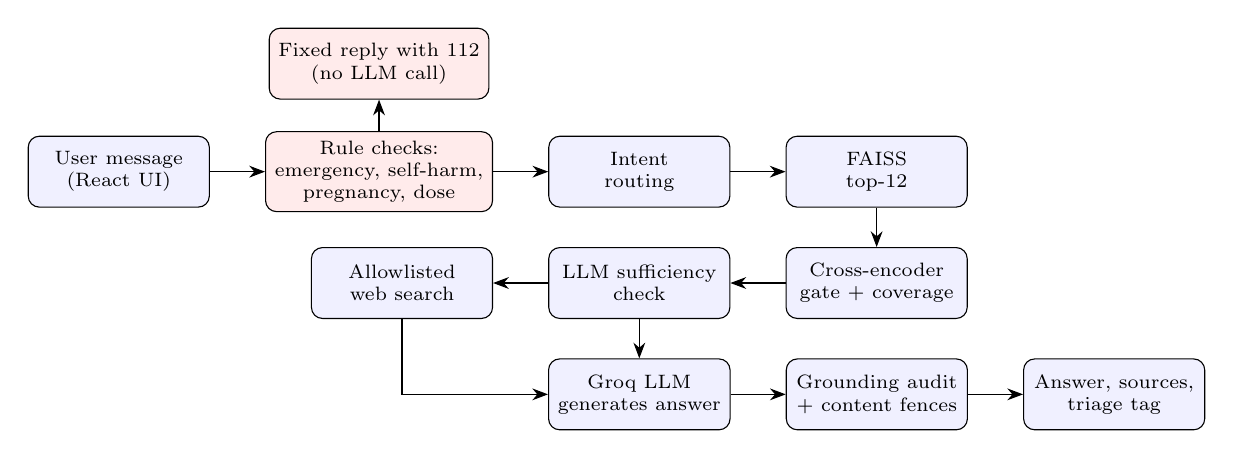
\begin{tikzpicture}[node distance=5mm and 7mm,
  box/.style={draw,rounded corners,align=center,font=\scriptsize,minimum height=9mm,minimum width=23mm,fill=blue!6},
  safe/.style={box,fill=red!8},
  arr/.style={-{Stealth[length=2mm]}}]
\node[box](u){User message\\(React UI)};
\node[safe,right=of u](e){Rule checks:\\emergency, self-harm,\\pregnancy, dose};
\node[box,right=of e](i){Intent\\routing};
\node[box,right=of i](r){FAISS\\top-12};
\node[box,below=of r](g){Cross-encoder\\gate + coverage};
\node[box,left=of g](s){LLM sufficiency\\check};
\node[box,left=of s](w){Allowlisted\\web search};
\node[box,below=of s](gen){Groq LLM\\generates answer};
\node[box,right=of gen](v){Grounding audit\\+ content fences};
\node[box,right=of v](o){Answer, sources,\\triage tag};
\node[safe,above=of e,yshift=-1mm](f){Fixed reply with 112\\(no LLM call)};
\draw[arr](u)--(e);\draw[arr](e)--(i);\draw[arr](i)--(r);\draw[arr](r)--(g);
\draw[arr](g)--(s);\draw[arr](s)--(w);\draw[arr](s)--(gen);\draw[arr](w)|-(gen);
\draw[arr](gen)--(v);\draw[arr](v)--(o);\draw[arr](e)--(f);
\end{tikzpicture}
\caption{Online answering path. Red boxes run without a language-model call. Social and off-topic messages are answered by fixed text after intent routing and are omitted for clarity.}
\label{fig:overview}
\end{figure}

\subsection{Knowledge Base}
The knowledge base is the directory \code{backend/data/raw\_docs}. A registry file (\code{SOURCES.md}) records, for every document, the publisher, source URL, review date and the first 16 hexadecimal characters of its SHA-256 hash; the ingestion script refuses any file that is not listed or whose hash prefix does not match. The corpus has 32 documents (24 PDFs and 8 text files). By publisher label in the registry, 24 are attributed to WHO and the remaining eight to Ministry of Health and Family Welfare (MoHFW), ICMR, National Health Mission or the Central TB Division sources, with several jointly labelled (Table~\ref{tab:corpus}). Topics include dengue, malaria, tuberculosis, HIV, hepatitis B, meningitis, COVID-19, pneumonia and diarrhoea, diabetes and hypertension, cardiovascular disease, anaemia, obesity, nutrition and physical activity, mental health (anxiety, depression, stress), maternal and child health, air pollution and flood-related health guidance. Eight documents are plain-text files, several of them short summaries rather than full guidelines (the smallest produce only 8 to 15 chunks; for example, the dengue entry is a text summary of a WHO fact sheet). A separate file lists conditions known to be missing from the corpus (\code{uncovered\_conditions.json}); these questions are routed to the web fallback.

\begin{table}[t]
\centering\small
\caption{Composition of the knowledge base by registry publisher label (counts from \code{SOURCES.md}).}
\label{tab:corpus}
\begin{tabular}{lr}
\toprule
Publisher label & Documents\\
\midrule
WHO & 24\\
MoHFW India & 3\\
ICMR / MoHFW; MoHFW / WHO; WHO / ILO; WHO / UNICEF; CTD / MoHFW & 1 each (5)\\
\midrule
Total (24 PDF + 8 text files) & 32\\
\bottomrule
\end{tabular}
\end{table}

\subsection{Document Processing, Embeddings and Index}
PDFs are read with \code{pypdf}; text files are read directly. A custom chunker accumulates text until a size of 500 characters is reached and carries 50 characters of overlap into the next chunk. The measured mean chunk length in the committed index is 594 characters (computed by us from the metadata file). Chunks are embedded with \code{sentence-transformers/all-MiniLM-L6-v2} through the FastEmbed ONNX runtime on CPU, producing 384-dimensional vectors that are L2-normalised and stored in a FAISS \code{IndexFlatIP}. The committed index contains 24,800 vectors with matching metadata rows across all 32 documents; the count is unequal between documents (from 8 chunks for the shortest text summary to 7,694 for the WHO air-quality guideline PDF), so document-level coverage by chunk count should not be read as coverage by topic. At start-up, an integrity check compares the source registry with the index and, in \code{strict} mode, stops the service if they disagree.

\subsection{Intent Routing and Safety Rules}
Intent is determined by regular expressions before any model call: greetings, thanks, goodbyes and small talk receive short fixed replies; clearly off-topic requests (for example, code or a stock price) receive a polite redirect; everything else defaults to the health route. Separate regular-expression paths detect (i) explicit first-person self-harm or overdose statements, (ii) acute red flags such as severe chest pain with warning signs, trouble breathing, heavy bleeding, unconsciousness, stroke signs and anaphylaxis, expressed in the present or personal tense (informational questions such as ``what are the symptoms of\ldots'' are exempted), (iii) fever in a newborn or an infant under three months, (iv) a fall or broken waters during pregnancy, and (v) requests for exact medicine doses. Cases (i)--(iii) return a fixed reply that tells the user to call 112 (and, for self-harm, to call the Tele-MANAS helpline, configured by default as 14416) and attach official-resource sources; case (iv) returns a fixed maternity-urgent reply; case (v) returns a fixed refusal that refers the user to a doctor or pharmacist. None of these paths calls the LLM. If no rule fires, a small LLM call may label urgency, but an ``emergency'' label from the model is deliberately downgraded to ``consult soon'': only an explicit rule may create the emergency response. The rules are English-centred and heuristic; we did not evaluate their recall.

\subsection{Retrieval and the Relevance Gate}\label{sec:gate}
For a health question, the query (concatenated with up to two prior user turns when the question refers back to the conversation) is embedded and the 12 nearest chunks are retrieved. Chunks scoring below a retrieval floor of 0.45 are dropped. The remaining (query, chunk) pairs are scored by the cross-encoder \code{Xenova/ms-marco-MiniLM-L-6-v2}; chunks whose source label names a condition the user did not ask about are removed. The decision function then combines the signals: the effective cross-encoder threshold is the maximum of a hard safety floor ($-9.5$), the configured global value, a calibrated global value and a per-document value, and a coverage registry marks named conditions as covered or uncovered. The outcome is one of \textsc{answer} (use local passages), \textsc{general} (a health-related question the corpus cannot support) or \textsc{off\_topic}. If the cross-encoder fails to load or errors, the gate fails closed. For accepted queries the top four reranked passages (six for comparison questions) are kept, and an LLM sufficiency call checks that they contain the specific facts requested; if not, the web fallback is used.

\subsection{Web Fallback, Generation and Verification}
The web fallback queries DuckDuckGo with \code{site:} filters for nine allowlisted hosts (who.int, mohfw.gov.in, icmr.gov.in, nhp.gov.in, nhm.gov.in, cdc.gov, nhs.uk, medlineplus.gov, nih.gov), re-checks each URL against the allowlist, does not follow redirects, limits the downloaded body to 512 KB, reranks page passages with the cross-encoder and caches results for one hour. Generation uses Groq-hosted models: the default is \code{qwen/qwen3.8-27b} with fallback to \code{openai/gpt-oss-120b} and \code{openai/gpt-oss-20b} when a model is rate-limited (a three-minute per-model cooldown), and the smaller model is used for educational questions. A whole chat request has a 25 s budget. The prompt defines four answer modes (grounded, web-trusted, mixed, general) and forbids doses and schedules unless a supplied source states them. After generation, a deterministic lexical-overlap check flags sentences with little support in the evidence; flagged answers, and answers containing numeric or medication claims absent from the sources, are reviewed by an LLM verifier (if enabled) or have the offending sentences removed. A separate grounding audit with a different model from the generator is also implemented. All of these checks are lexical or LLM-based and do not constitute proof of entailment.

\subsection{Health Tools and Application}
The backend is FastAPI with endpoints for chat, health status, warm-up, nearby hospitals and two admin-token-protected diagnostics (Appendix~\ref{app:config}). The BMI calculator computes weight divided by height squared and reports adult ranges (below 18.5, 18.5 to under 25, 25 to under 30, 30 or higher) for ages 20 and over, and declines to assign a category for ages 2--19 because age- and sex-specific percentiles are required. The Quick Help panel lists red-flag situations, a call-112 button and three preset questions. The Nearby Hospitals panel can open an entered place or PIN code in Google Maps, use the device's location, or request up to ten hospitals within 15 km through the backend, which calls the Geoapify geocoding and places services with a server-side key; without that key the endpoint returns an error and the panel still offers Maps. Voice input uses the browser's speech recognition with the \code{en-IN} language setting, and replies are revealed word by word with a ``Show full reply'' control. The frontend is React~19 with Vite and Tailwind~CSS; the backend is deployed separately (Section~\ref{sec:deploy}).

\subsection{Deployment}\label{sec:deploy}
The repository contains a Vercel configuration for the frontend, a Render service definition and a Dockerfile (port 7860, with Hugging Face Spaces metadata in the README) for the backend. The production frontend build calls a hard-coded Render URL; the development build reads an environment variable. We did not verify which hosting targets are currently live.

\subsection{Privacy Behaviour as Implemented}\label{sec:privacy}
The backend does not store conversations. Each request carries the current question and up to six recent turns to the LLM provider; web searches may be sent to the search provider and the fetched sites; browser voice recognition may be processed by the browser vendor. The backend does record aggregates in SQLite or, if configured, Postgres: for refusals, a PII-scrubbed (regular-expression) normalised topic text of at most 180 characters with counts and scores, and for answers, a hash of that topic, answer mode, gate scores and a timestamp. User identifiers are salted-hash values (the frontend sends the constant \code{anonymous}). Scrubbing is heuristic and cannot remove all identifying text. The interface tells users not to share identifying details.

\subsection{Evaluation Protocol}
The repository contains a \emph{gate-only} benchmark (\code{backend/eval}). A seeded generator (seed 20261104) produces 430 queries from templates: in-corpus queries are made by filling templates (English, Hinglish and mixed) with topics or section headings taken from the chunk metadata; near-domain uncovered queries use condition names from the uncovered-conditions registry; the remaining queries are generic out-of-domain requests and small talk. There are 300 calibration and 130 test queries; the test split has 45 in-corpus, 45 near-domain uncovered, 28 out-of-domain and 12 small-talk queries (90 English, 28 Hinglish, 12 mixed). The runner compares four baselines (a retrieval-score threshold; a global cross-encoder threshold; an earlier midpoint-keyword gate; and always answering with the LLM and no retrieval), the multi-signal gate, and three ablations (no cluster thresholds, no coverage registry, no auto-calibration). Metrics are the false-answer rate on near-domain uncovered queries, the false-refusal rate on in-corpus queries, and the share of health queries answered from the corpus. Latency is measured for retrieval plus cross-encoder only. Software checks are described in Section~\ref{sec:software}.

\begin{table}[t]
\centering\small
\caption{Computing environment. The first block is taken from repository configuration; the last row is the environment in which we re-ran the software checks.}
\label{tab:env}
\begin{tabular}{p{3.6cm}p{11cm}}
\toprule
Item & Value\\
\midrule
Embeddings & all-MiniLM-L6-v2 via FastEmbed (ONNX, CPU), 384 dimensions\\
Vector index & FAISS \code{IndexFlatIP}, 24,800 vectors\\
Reranker & \code{Xenova/ms-marco-MiniLM-L-6-v2} (ONNX, CPU)\\
LLM & Groq-hosted \code{qwen/qwen3.8-27b} (default), \code{openai/gpt-oss-120b}, \code{openai/gpt-oss-20b}\\
Backend & Python 3.11 (Docker), FastAPI, FAISS, pypdf\\
Frontend & React 19, Vite 8, Tailwind CSS 3, axios\\
Checks run for this paper & Python 3.13, Node 22, Linux sandbox, 2026-11-15\\
\bottomrule
\end{tabular}
\end{table}

%------------------------------------------------------------------
\section{Results}
\subsection{Corpus Coverage}
All 32 registered documents are present in the committed index (verified with the repository's index check on 2026-11-15). Coverage is uneven: malaria and tuberculosis have two registered documents each and dengue has one short text summary, and many other topics rely on a single fact sheet or summary, and chunk counts range from 8 to 7,694 per document. Conditions outside the corpus (for example tetanus appears as a near-domain uncovered example in the benchmark) must be answered from the web or from general knowledge. We did not measure the share of real user questions the corpus covers.

\subsection{Gate-Only Benchmark}
Table~\ref{tab:gate} shows the committed results on the 130-query test split, and Appendix~\ref{app:gate} gives all systems. The final multi-signal gate accepted none of the 45 near-domain uncovered queries (0/45, 95\% Wilson interval 0--7.9\%) and none of the 85 non-corpus queries overall (0/85, 0--4.3\%), but it also refused 24 of 45 in-corpus queries (53.3\%, 39--67\%); it answered 21 of the 90 health queries (23.3\%, 16--33\%) from local passages. A permissive retrieval-score threshold answered 41 of 45 in-corpus queries but also accepted 82.2\% of near-domain uncovered queries; always answering with the LLM and no retrieval accepted all of them. Removing the coverage registry raised the false-answer rate to 48.9\%, while removing auto-calibration changed the false-refusal rate from 53.3\% to 46.7\% with no false answers (Appendix~\ref{app:gate}). Measured gate latency (retrieval plus cross-encoder, excluding LLM and network) was 233 ms at the median and 3,703 ms at the 95th percentile; it is reported in the metadata as a local proxy because it used a cached sentence-transformers adapter instead of the production FastEmbed runtime.

\begin{table}[t]
\centering\small
\caption{Gate-only results on the 130-query test split (committed \code{results.json}; Wilson intervals computed by us). A gate non-answer may still lead to a web or general LLM answer.}
\label{tab:gate}
\begin{tabular}{lrrr}
\toprule
Measure & Count & Rate (\%) & 95\% CI (\%)\\
\midrule
Near-domain uncovered queries accepted (false answers) & 0/45 & 0.0 & 0--7.9\\
Non-corpus queries accepted (all classes) & 0/85 & 0.0 & 0--4.3\\
In-corpus queries refused (false refusals) & 24/45 & 53.3 & 39--67\\
In-corpus queries answered from corpus & 21/45 & 46.7 & 33--61\\
Health queries answered from corpus (in-corpus + near-domain) & 21/90 & 23.3 & 16--33\\
\bottomrule
\end{tabular}
\end{table}

\subsection{Software Checks}\label{sec:software}
We re-ran the repository's deterministic checks on 2026-11-15 (Table~\ref{tab:checks}). The earlier status note in the repository (dated 2026-11-04) reported 15 tests and an index of 3,341 vectors that was missing two documents; these figures are out of date, since the committed index now has 24,800 vectors covering all 32 documents. The retrieval smoke test, the end-to-end evaluation script and the other \code{test\_*.py} scripts need a model download, an LLM key or network access and were not run. There is no continuous-integration workflow in the repository.

\begin{table}[t]
\centering\small
\caption{Automated checks re-run for this paper (2026-11-15).}
\label{tab:checks}
\begin{tabular}{p{9.5cm}l}
\toprule
Check & Result\\
\midrule
\code{unittest discover -p "test\_quality*.py"} (offline) & 24 tests passed\\
\code{verify\_sources.py} (registry and SHA-256) & 32/32 documents match\\
\code{verify\_sources.py --check-index} & 24,800 vectors, all 32 documents indexed\\
Frontend \code{npm run lint} and \code{npm run build} & passed\\
\bottomrule
\end{tabular}
\end{table}

\subsection{Inconsistencies Found}
Reading the repository against its documentation surfaced several issues, summarised in Table~\ref{tab:defects}. They concern documentation or evidence rather than answer quality, but each affects how far the reported numbers can be trusted.

\begin{table}[t]
\centering\small
\caption{Inconsistencies between documentation, configuration and code found while preparing this paper.}
\label{tab:defects}
\begin{tabular}{p{5.2cm}p{9.3cm}}
\toprule
Finding & Detail\\
\midrule
Status note out of date & The 2026-11-04 note reported 15 tests and a 3,341-vector index missing two documents; the repository now shows 24 tests and a complete 24,800-vector index.\\
Python version & The README stated Python 3.10; the code uses \code{enum.StrEnum}, which needs 3.11 (the Dockerfile uses 3.11). Vite 8 also requires Node 20.19 or 22.12 and later.\\
Frontend API URL & The environment example suggests setting the API URL in the hosting dashboard, but the production build ignores it and uses a hard-coded URL.\\
Runtime thresholds vs.\ benchmark & The committed runtime threshold file holds a single global entry at $-10.0$ (so the $-9.5$ floor is what applies), with 190 calibration and 82 test samples, whereas the benchmark metadata reports 300 and 130 samples and a calibrated baseline cross-encoder threshold of $-2.93$. We could not determine whether the deployed gate reproduces the benchmark's gate.\\
Noisy template queries & Some generated in-corpus queries are low quality, for example one built from a chunk heading that is a statistical fragment (query Q0003: ``What does the guidance say about (CI 95\% 0.16 --- 0.36)?''), which likely inflates the false-refusal rate.\\
Stub tools & The outbreak-alert function returns a fixed placeholder; no live surveillance feed is connected.\\
\bottomrule
\end{tabular}
\end{table}

%------------------------------------------------------------------
\section{Discussion}
\textbf{What the evidence supports.} The repository supports the claim that the system implements layered controls: deterministic safety paths, a fail-closed relevance gate, a source-hash-checked corpus and a post-generation content fence. The benchmark supports a narrower claim: on template-generated queries the final gate is conservative, never accepting an uncovered near-domain query, at the price of refusing about half of the in-corpus queries. Such a refusal does not leave the user without an answer, because the system then falls back to allowlisted web pages or a general-health answer, but those answers are less tightly grounded than corpus answers, and we have no measurement of their correctness.

\textbf{Gate design.} The benchmark illustrates the usual trade-off: a retrieval-score threshold accepts most in-corpus queries but also most near-domain ones, since passages about a related condition look similar to the question; a cross-encoder threshold alone sits in between; coverage knowledge removes the near-domain false answers. The final gate's low in-corpus acceptance suggests the thresholds are too strict for the template queries, and the noisy queries noted above may partly explain this; a hand-written test set would be more informative.

\textbf{Safety policy.} The dose fence and the rule that a model cannot create an emergency banner are judgement calls. They favour caution over helpfulness and rely on a clinician-reviewed policy that does not yet exist; clinicians might draw these lines differently.

\textbf{Responsible use.} The system is a health-information tool, not a medical device. It does not diagnose, does not prescribe, and displays the emergency number prominently, consistent with the transparency and safety principles of WHO guidance \citep{who2021}. None of its content or behaviour has been reviewed by a clinician.

\textbf{Threats to validity.} \emph{Internal:} benchmark queries are generated by templates from the same index they test, and the labels follow from the generator rather than from human judgement; the committed results used a proxy embedding adapter; thresholds in the runtime file differ from those described in the benchmark. \emph{Construct:} the benchmark measures only the answer/refuse decision, not whether an answer is correct, complete or safe, and the lexical support check can accept an unsupported sentence that reuses the right words. \emph{External:} the sources are WHO and Indian government documents; the benchmark has English, Hinglish and mixed templates but no real users, voice input or regional-language text. The LLM providers and model names change over time, so results may not be repeatable.

\textbf{Limitations.}
(i) No clinician review, clinical validation, usability study or real-user evaluation.
(ii) No end-to-end answer-quality, hallucination, emergency-recall or dose-leak measurement exists in the repository.
(iii) Hindi and Hinglish are handled only by prompts and by a few keyword rules; voice input is English only.
(iv) Corpus coverage is uneven and static, and some documents are short summaries.
(v) The emergency rules are regular expressions and will miss phrasings they do not match.
(vi) Web fallback quality depends on search results and page structure; hosted-LLM rate limits can trigger model fallback or a busy response.
(vii) The backend has no rate limiting or authentication for chat, and the default CORS origin is open.

\textbf{Future work.} Priorities are a hand-written, clinician-reviewed evaluation set including emergencies, dose requests and Hindi/Hinglish messages; an end-to-end evaluation with human grading and entailment checks; reconciling the deployed gate thresholds with the benchmark; a local multilingual emergency classifier that does not depend on rules alone; continuous integration; rate limiting; and a user study.

%------------------------------------------------------------------
\section{Conclusion}
SwasthyaSaathi combines a hash-verified WHO and Indian government corpus, a multi-signal relevance gate, deterministic emergency, self-harm and dose paths, an allowlisted web fallback, and a grounding and content-fence pass in a public-health information chatbot with a small set of health tools. The evidence in the repository shows that the software checks pass and that the final gate never accepted an uncovered near-domain query on its template benchmark while refusing about half of the in-corpus queries. It does not yet show answer correctness, emergency recall or user benefit. The system needs clinician review, a hand-written multilingual evaluation and field testing before any real deployment.

\section*{Author Contributions}
[To be completed by the authors: each author's role in the conception, implementation, evaluation and writing.]

\section*{Use of AI Tools}
This manuscript was drafted with the assistance of an AI assistant (Claude, by Anthropic), which inspected the project repository, re-ran the automated checks described in Section~\ref{sec:software} and computed the derived statistics in this paper from the repository files. The authors are responsible for reviewing, correcting and approving all content. [The authors should state here any AI assistance used in writing the software itself, which cannot be determined from the repository.] The hosted LLMs used by the system are described in the Methods.

\section*{Acknowledgments}
[To be completed by the authors.] We acknowledge the publishers of the WHO and Government of India documents used as the knowledge base.

\section*{Data and Code Availability}
The code, evaluation scripts, committed benchmark results and source registry are available at \url{https://github.com/shreyaaaah/SwasthyaSaathi}. The source documents belong to their publishers; the registry lists their addresses and review dates.

%------------------------------------------------------------------
\begin{thebibliography}{99}\small
\setlength{\itemsep}{2pt}

\bibitem[Asai et al.(2024)]{asai2024}
Asai, A., Wu, Z., Wang, Y., Sil, A., and Hajishirzi, H. (2024). Self-RAG: Learning to retrieve, generate, and critique through self-reflection. In \emph{The Twelfth International Conference on Learning Representations (ICLR)}.

\bibitem[Bajaj et al.(2016)]{bajaj2016}
Bajaj, P., Campos, D., Craswell, N., Deng, L., Gao, J., Liu, X., et al. (2016). MS MARCO: A human generated machine reading comprehension dataset. arXiv preprint arXiv:1611.09268.

\bibitem[Brown et al.(2001)]{brown2001}
Brown, L. D., Cai, T. T., and DasGupta, A. (2001). Interval estimation for a binomial proportion. \emph{Statistical Science} 16, 101--133.

\bibitem[Es et al.(2024)]{es2024}
Es, S., James, J., Espinosa-Anke, L., and Schockaert, S. (2024). RAGAs: Automated evaluation of retrieval augmented generation. In \emph{Proceedings of the 18th Conference of the European Chapter of the Association for Computational Linguistics: System Demonstrations}.

\bibitem[Gao et al.(2023)]{gao2023}
Gao, Y., Xiong, Y., Gao, X., Jia, K., Pan, J., Bi, Y., et al. (2023). Retrieval-augmented generation for large language models: A survey. arXiv preprint arXiv:2312.10997.

\bibitem[Greshake et al.(2023)]{greshake2023}
Greshake, K., Abdelnabi, S., Mishra, S., Endres, C., Holz, T., and Fritz, M. (2023). Not what you've signed up for: Compromising real-world LLM-integrated applications with indirect prompt injection. In \emph{Proceedings of the 16th ACM Workshop on Artificial Intelligence and Security (AISec)}.

\bibitem[Ji et al.(2023)]{ji2023}
Ji, Z., Lee, N., Frieske, R., Yu, T., Su, D., Xu, Y., et al. (2023). Survey of hallucination in natural language generation. \emph{ACM Computing Surveys} 55(12), Article 248.

\bibitem[Johnson et al.(2019)]{johnson2019}
Johnson, J., Douze, M., and J{\'e}gou, H. (2019). Billion-scale similarity search with GPUs. \emph{IEEE Transactions on Big Data} 7, 535--547.

\bibitem[Joshi et al.(2020)]{joshi2020}
Joshi, P., Santy, S., Budhiraja, A., Bali, K., and Choudhury, M. (2020). The state and fate of linguistic diversity and inclusion in the NLP world. In \emph{Proceedings of the 58th Annual Meeting of the Association for Computational Linguistics}.

\bibitem[Karpukhin et al.(2020)]{karpukhin2020}
Karpukhin, V., Oguz, B., Min, S., Lewis, P., Wu, L., Edunov, S., Chen, D., and Yih, W. (2020). Dense passage retrieval for open-domain question answering. In \emph{Proceedings of EMNLP 2020}, 6769--6781.

\bibitem[Laranjo et al.(2018)]{laranjo2018}
Laranjo, L., Dunn, A. G., Tong, H. L., Kocaballi, A. B., Chen, J., Bashir, R., et al. (2018). Conversational agents in healthcare: a systematic review. \emph{Journal of the American Medical Informatics Association} 25, 1248--1258.

\bibitem[Lewis et al.(2020)]{lewis2020}
Lewis, P., Perez, E., Piktus, A., Petroni, F., Karpukhin, V., Goyal, N., et al. (2020). Retrieval-augmented generation for knowledge-intensive NLP tasks. In \emph{Advances in Neural Information Processing Systems (NeurIPS)}, vol.~33, 9459--9474.

\bibitem[Nogueira and Cho(2019)]{nogueira2019}
Nogueira, R., and Cho, K. (2019). Passage re-ranking with BERT. arXiv preprint arXiv:1901.04085.

\bibitem[Perez and Ribeiro(2022)]{perez2022}
Perez, F., and Ribeiro, I. (2022). Ignore previous prompt: Attack techniques for language models. arXiv preprint arXiv:2211.09527.

\bibitem[Reimers and Gurevych(2019)]{reimers2019}
Reimers, N., and Gurevych, I. (2019). Sentence-BERT: Sentence embeddings using Siamese BERT-networks. In \emph{Proceedings of EMNLP-IJCNLP 2019}, 3982--3992.

\bibitem[Shuster et al.(2021)]{shuster2021}
Shuster, K., Poff, S., Chen, M., Kiela, D., and Weston, J. (2021). Retrieval augmentation reduces hallucination in conversation. In \emph{Findings of the Association for Computational Linguistics: EMNLP 2021}.

\bibitem[Singhal et al.(2023)]{singhal2023}
Singhal, K., Azizi, S., Tu, T., Mahdavi, S. S., Wei, J., Chung, H. W., et al. (2023). Large language models encode clinical knowledge. \emph{Nature} 620, 172--180.

\bibitem[Thirunavukarasu et al.(2023)]{thirunavukarasu2023}
Thirunavukarasu, A. J., Ting, D. S. J., Elangovan, K., Gutierrez, L., Tan, T. F., and Ting, D. S. W. (2023). Large language models in medicine. \emph{Nature Medicine} 29, 1930--1940.

\bibitem[Tudor Car et al.(2020)]{tudorcar2020}
Tudor Car, L., Dhinagaran, D. A., Kyaw, B. M., Kowatsch, T., Joty, S., Theng, Y.-L., and Atun, R. (2020). Conversational agents in health care: Scoping review and conceptual analysis. \emph{Journal of Medical Internet Research} 22, e17158.

\bibitem[Wang et al.(2020)]{wang2020}
Wang, W., Wei, F., Dong, L., Bao, H., Yang, N., and Zhou, M. (2020). MiniLM: Deep self-attention distillation for task-agnostic compression of pre-trained transformers. In \emph{Advances in Neural Information Processing Systems (NeurIPS)}, vol.~33, 5776--5788.

\bibitem[Wilson(1927)]{wilson1927}
Wilson, E. B. (1927). Probable inference, the law of succession, and statistical inference. \emph{Journal of the American Statistical Association} 22, 209--212.

\bibitem[World Health Organization(2021)]{who2021}
World Health Organization (2021). \emph{Ethics and governance of artificial intelligence for health: WHO guidance}. Geneva: World Health Organization.

\bibitem[Xiong et al.(2024)]{xiong2024}
Xiong, G., Jin, Q., Lu, Z., and Zhang, A. (2024). Benchmarking retrieval-augmented generation for medicine. In \emph{Findings of the Association for Computational Linguistics: ACL 2024}.

\bibitem[Zakka et al.(2024)]{zakka2024}
Zakka, C., Shad, R., Chaurasia, A., Dalal, A. R., Kim, J. L., Moor, M., et al. (2024). Almanac: Retrieval-augmented language models for clinical medicine. \emph{NEJM AI} 1(2).

\bibitem[Ministry of Home Affairs(n.d.)]{erss}
Ministry of Home Affairs, Government of India (n.d.). Emergency Response Support System (ERSS). \url{https://www.mha.gov.in/emergency-response-support-system-erss} (accessed 2026).

\bibitem[Ministry of Health and Family Welfare(n.d.)]{nmhp}
Directorate General of Health Services, Ministry of Health and Family Welfare, Government of India (n.d.). National Mental Health Programme (including Tele-MANAS). \url{https://www.dghs.mohfw.gov.in/national-mental-health-programme.php} (accessed 2026).

\bibitem[SwasthyaSaathi(2026)]{sources}
SwasthyaSaathi repository (2026). \code{backend/data/raw\_docs/SOURCES.md}: knowledge-base provenance registry. \url{https://github.com/shreyaaaah/SwasthyaSaathi}.

\end{thebibliography}

%------------------------------------------------------------------
\appendix
\section{Gate Benchmark: All Systems}\label{app:gate}
\begin{table}[h]
\centering\small
\caption{All systems on the 130-query test split, from the committed \code{eval/RESULTS.md} and \code{results.json}. FA = false-answer rate on near-domain uncovered queries (45); FR = false-refusal rate on in-corpus queries (45); ``Health answered'' = share of the 90 in-corpus and near-domain queries answered from local passages. Latency columns are identical for all systems because they were measured once for retrieval plus cross-encoder.}
\begin{tabular}{lrrrr}
\toprule
System & FA & FR & Health answered & Gate non-answer (\%)\\
\midrule
B0 retrieval-score threshold & 0.822 & 0.089 & 0.867 & 34.6\\
B1 global cross-encoder threshold & 0.511 & 0.489 & 0.511 & 64.6\\
B2 original midpoint keyword gate & 0.400 & 0.956 & 0.222 & 84.6\\
B3 always LLM, no retrieval & 1.000 & 0.000 & 1.000 & 30.8\\
Multi-signal gate (final) & 0.000 & 0.533 & 0.233 & 83.8\\
\; Ablation: no cluster thresholds & 0.000 & 0.533 & 0.233 & 83.8\\
\; Ablation: no coverage registry & 0.489 & 0.533 & 0.478 & 66.9\\
\; Ablation: no auto-calibration & 0.000 & 0.467 & 0.267 & 79.2\\
\bottomrule
\end{tabular}
\end{table}
Confusion counts for the final gate (in-corpus is positive): TP 21, FP 0, FN 24, TN 85. Latency (retrieval plus cross-encoder, median/95th percentile): 233.4 ms / 3,702.6 ms.

\section{System Configuration}\label{app:config}
\begin{table}[h]
\centering\small
\caption{Main settings taken from the code and configuration files.}
\begin{tabular}{p{4cm}p{10.5cm}}
\toprule
Item & Value\\
\midrule
Chunking & 500 characters, 50 overlap, custom splitter; PDFs read with \code{pypdf}\\
Index & FAISS \code{IndexFlatIP}, L2-normalised 384-dimensional vectors, 24,800 chunks\\
Retrieval & top 12 candidates; floor 0.45; top 4 passages kept (6 for comparisons)\\
Gate & hard cross-encoder floor $-9.5$; per-document and calibrated thresholds; coverage registry; fail-closed\\
LLM chain & \code{qwen/qwen3.8-27b}, \code{openai/gpt-oss-120b}, \code{openai/gpt-oss-20b}; 8 s per call; 25 s per request\\
Caches & answer cache 256 entries, 24 h; web cache 3,600 s\\
History & up to 8 turns accepted by the API, 6 used; 2,000 characters per message\\
Web allowlist & who.int, mohfw.gov.in, icmr.gov.in, nhp.gov.in, nhm.gov.in, cdc.gov, nhs.uk, medlineplus.gov, nih.gov\\
Emergency number & 112 (default); Tele-MANAS 14416 (default configuration value)\\
Endpoints & \code{GET /}, \code{/health}, \code{/warmup}; \code{POST /chat} (aliases \code{/api/chat}, \code{/api/query}), \code{/hospitals/nearby}; admin-token: \code{GET /latency}, \code{/admin/knowledge-gaps}\\
\bottomrule
\end{tabular}
\end{table}

\section{Chat Response Format}
The chat endpoint returns \code{answer}, \code{sources} (document name, section, snippet of up to 300 characters, score, source type, URL), \code{is\_grounded}, \code{triage\_tag} (\textsc{emergency}, \textsc{maternity\_urgent}, \textsc{consult\_soon}, \textsc{self\_care} or \textsc{general\_info}), \code{tools\_used}, \code{response\_time\_ms}, \code{gate\_decision}, \code{answer\_mode} (\textsc{grounded}, \textsc{web\_trusted}, \textsc{mixed}, \textsc{general} or \textsc{social}), \code{gate\_scores}, \code{intent} and \code{emergency\_contact}.

\section{Safety Behaviour Enforced in Code}
\begin{enumerate}[leftmargin=*]
  \item Explicit self-harm or overdose statements, acute red flags, infant fever and pregnancy danger events are handled by fixed replies without an LLM call; the self-harm reply names 112 and the Tele-MANAS helpline (sources: \citealt{erss}, \citealt{nmhp}).
  \item Requests for exact doses receive a fixed referral to a clinician or pharmacist.
  \item The LLM may not create an emergency response by itself; its ``emergency'' label is downgraded to ``consult soon''.
  \item The relevance gate fails closed when the reranker is unavailable.
  \item Numeric and medication claims not present in the supplied evidence are removed or reviewed before display.
  \item Retrieved text and user text are marked as untrusted in the sufficiency, triage and verifier prompts.
  \item Web results must come from allowlisted hosts; redirects are not followed.
  \item Conversations are not stored; aggregate topic and decision metadata may be (Section~\ref{sec:privacy}).
\end{enumerate}
No clinician has reviewed these rules.

\section{Reproducibility Checklist}
\begin{table}[h]
\centering\small
\caption{Reproducibility checklist.}
\begin{tabular}{p{3.6cm}p{11cm}}
\toprule
Item & Information\\
\midrule
Corpus & 32 documents (24 PDF, 8 text), 24,800 chunks; registry with URLs, dates and SHA-256 prefixes in \code{backend/data/raw\_docs/SOURCES.md} \citep{sources}\\
Benchmark & \code{backend/eval/generate\_dataset.py} (seed 20261104), \code{queries.jsonl} (430 queries), \code{run\_gate\_eval.py}, \code{results.json}\\
Not re-run here & Gate benchmark; end-to-end evaluation; live scripts needing network, model downloads or LLM keys\\
Re-run here & 24 offline unit tests, source and index verification, frontend lint and build (2026-11-15)\\
Build & \code{pdflatex swasthyasaathi\_paper.tex} (twice) in \code{docs/paper}\\
\bottomrule
\end{tabular}
\end{table}

\end{document}
